\section{Evidencia en Niveles Indexados y Efecto Cicatriz (Scarring Effect)}

% ================================================================
\begin{frame}{Trayectoria Indexada ($\text{PIB}_{2019=100}$): Cicatriz en Enclaves}
\vspace{-0.18cm}
\begin{center}
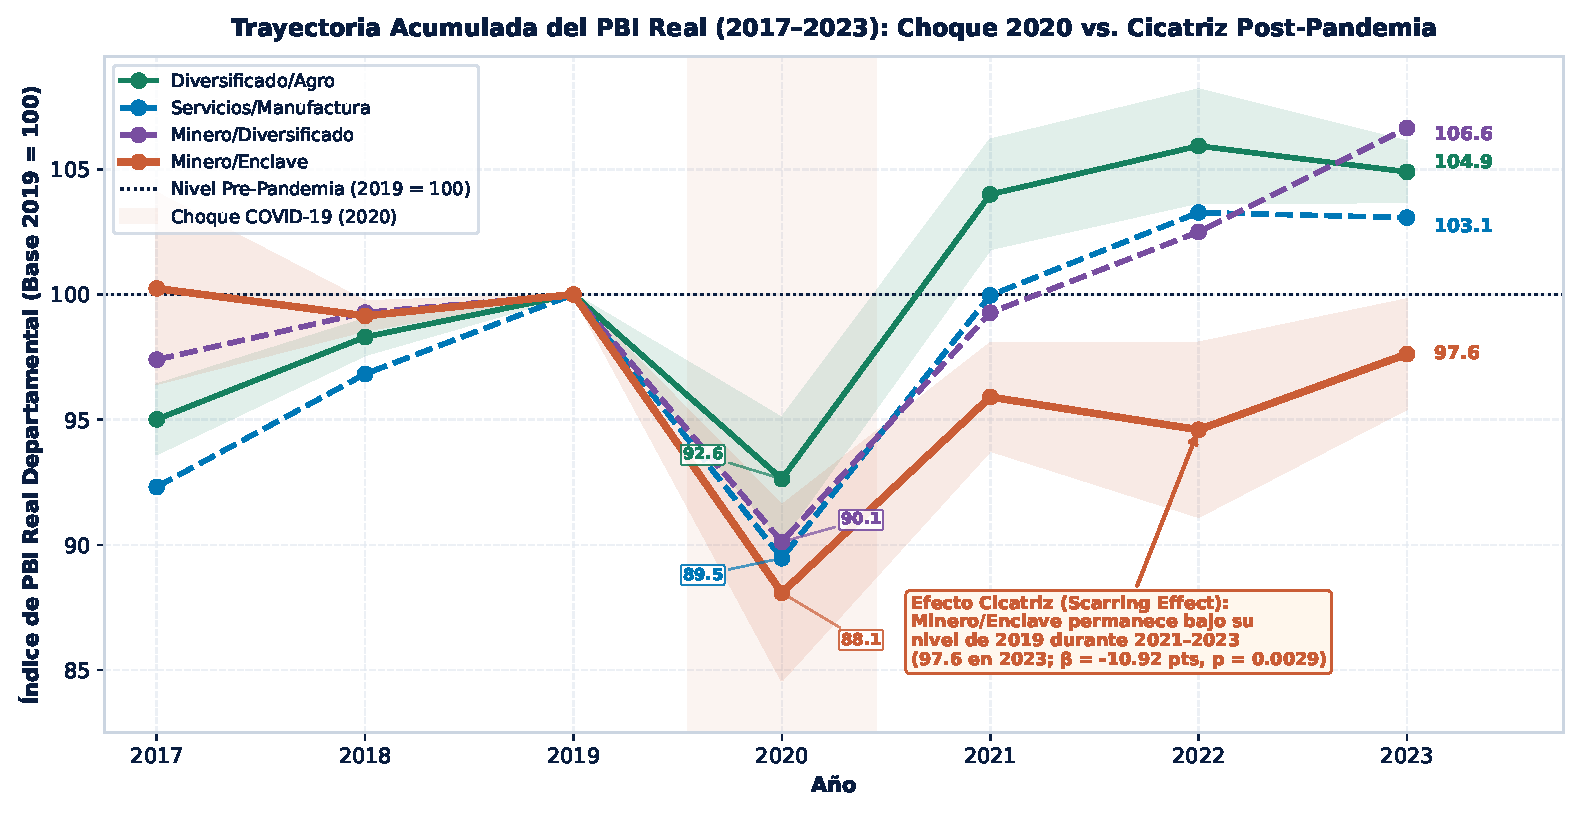
\includegraphics[width=0.86\textwidth,height=0.47\textheight,keepaspectratio]{figures/fig5_trayectoria_pib_indexado.pdf}
\end{center}
\vspace{-0.24cm}
\begin{columns}[T,onlytextwidth]
\begin{column}{0.58\textwidth}
\begin{ccdebox}[left=2mm,right=2mm,top=0.8mm,bottom=0.8mm]
\scriptsize\RaggedRight
\textbf{Divergencia 2021--2023}: \textit{Diversificado/Agro} ($104.9$), \textit{Minero/Div.} ($106.6$) y \textit{Serv./Manuf.} ($103.1$) superaron el nivel de 2019; \textbf{Minero/Enclave quedó bajo 100 todo el trienio ($95.9 \rightarrow 94.6 \rightarrow 97.6$)}.
\end{ccdebox}
\end{column}
\begin{column}{0.39\textwidth}
\begin{keybox}[left=2mm,right=2mm,top=0.8mm,bottom=0.8mm]
\scriptsize\RaggedRight \textbf{Mecanismo}: Conflictividad en el Corredor Minero y baja articulación local frenaron la recuperación.
\end{keybox}
\end{column}
\end{columns}
\source{Panel balanceado 2017--2023 ($N=24, T=7, \text{Obs}=168$). Elaboración propia (\texttt{generar\_analisis\_completo.py}).}
\end{frame}

% ================================================================
\begin{frame}{Modelos en Nivel Indexado (M5--M6): Cicatriz al 1\%}
\vspace{-0.14cm}
\begin{columns}[T,onlytextwidth]
\begin{column}{0.57\textwidth}
\begin{ccdebox}[left=2mm,right=2mm,top=1mm,bottom=1mm]
\scriptsize
\textbf{\textcolor{ccdenavy}{Dependiente: Índice de PIB Real ($\text{PIB}_{i,2019}=100$, 2017--2023)}}
\vspace{0.03cm}

\resizebox{\linewidth}{!}{%
\renewcommand{\arraystretch}{1.06}
\begin{tabular}{@{}l r r r r@{}}
\toprule
& \multicolumn{2}{c}{\textbf{M5: Clusters ($K=4$)}} & \multicolumn{2}{c}{\textbf{M6: Continuo ($\text{Minería}_z$)}} \\
\cmidrule(lr){2-3}\cmidrule(lr){4-5}
\textbf{Regresor (Efectos Fijos)} & \textbf{Beta} & \textbf{$p$-valor} & \textbf{Beta} & \textbf{$p$-valor} \\
\midrule
Intercepto (Senda Pre-COVID) & $97.71^{***}$ & 0.0000 & $97.71^{***}$ & 0.0000 \\
$\text{COVID}_{2020}$ (Ref: Div./Agro) & $-5.14^{***}$ & 0.0016 & $-7.83^{***}$ & 0.0000 \\
$\text{POST}_{2021\text{--}23}$ (Ref: Div./Agro) & $+7.17^{***}$ & 0.0000 & $+4.19^{**}$ & 0.0224 \\
\midrule
$\text{COVID}_{2020} \times \text{Serv./Manuf.}$ & $-1.77$ & 0.3318 & --- & --- \\
$\text{COVID}_{2020} \times \text{Minero/Div.}$ & $-3.63$ & 0.4655 & --- & --- \\
\rowcolor{warn!12}
$\text{COVID}_{2020} \times \text{Minero/Enclave}$ & \textcolor{warn}{$\mathbf{-6.57^{**}}$} & \textcolor{warn}{\textbf{0.0495}} & --- & --- \\
$\text{POST}_{2021\text{--}23} \times \text{Serv./Manuf.}$ & $-1.45$ & 0.5212 & --- & --- \\
$\text{POST}_{2021\text{--}23} \times \text{Minero/Div.}$ & $-3.26$ & 0.5694 & --- & --- \\
\rowcolor{warn!18}
$\text{POST}_{2021\text{--}23} \times \text{Minero/Enclave}$ & \textcolor{warn}{$\mathbf{-10.92^{***}}$} & \textcolor{warn}{\textbf{0.0029}} & --- & --- \\
\rowcolor{ccdelight!22}
$\text{COVID}_{2020} \times \text{Minería}_z$ (1 SD) & --- & --- & \textcolor{ccdeblue}{$\mathbf{-2.39^{*}}$} & \textcolor{ccdeblue}{\textbf{0.0891}} \\
\rowcolor{ccdelight!22}
$\text{POST}_{2021\text{--}23} \times \text{Minería}_z$ (1 SD) & --- & --- & \textcolor{ccdeblue}{$\mathbf{-2.76^{*}}$} & \textcolor{ccdeblue}{\textbf{0.0747}} \\
\midrule
Observaciones / Departamentos & \multicolumn{2}{c}{168 / 24} & \multicolumn{2}{c}{168 / 24} \\
$R^2$ Within & \multicolumn{2}{c}{\textcolor{okgreen}{\textbf{0.3554}}} & \multicolumn{2}{c}{\textcolor{okgreen}{\textbf{0.3451}}} \\
Test $F$ Poolability ($p$-valor) & \multicolumn{2}{c}{\textbf{3.14 ($p < 0.0001$)}} & \multicolumn{2}{c}{\textbf{3.29 ($p < 0.0001$)}} \\
\bottomrule
\end{tabular}%
}
\end{ccdebox}
\end{column}

\begin{column}{0.40\textwidth}
\begin{contrastbox}{okgreen}{Salto Econométrico}
\scriptsize\RaggedRight
\begin{itemize}\setlength{\itemsep}{0.12em}
  \item \textbf{Efectos fijos validados:} El test de Poolability pasa de $p=0.51$ (en tasas) a \textbf{$p < 0.0001$} en niveles indexados.
  \item \textbf{Mayor ajuste:} El $R^2_{\text{within}}$ sube de $13.9\%$ a \textbf{$35.5\%$}.
  \item \textbf{Doble golpe al Enclave (M5):} Caída adicional de \textbf{$-6.57$ pts} en 2020 ($p=0.0495$) y rezago acumulado de \textbf{$-10.92$ pts} en 2021--2023 ($p=0.0029$).
  \item \textbf{Gradiente continuo (M6):} $+1\text{ SD}$ en minería reduce el nivel pospandemia en \textbf{$-2.76$ pts} ($p=0.075$).
\end{itemize}
\end{contrastbox}
\end{column}
\end{columns}
\source{Estimaciones PanelOLS con efectos fijos de entidad y errores estándar clusterizados (\texttt{resumen\_modelos\_econometricos.xlsx}).}
\end{frame}

% ================================================================
\begin{frame}{Contraste de Modelos: Tasas Anuales vs. Niveles}
\vspace{-0.18cm}
\begin{center}
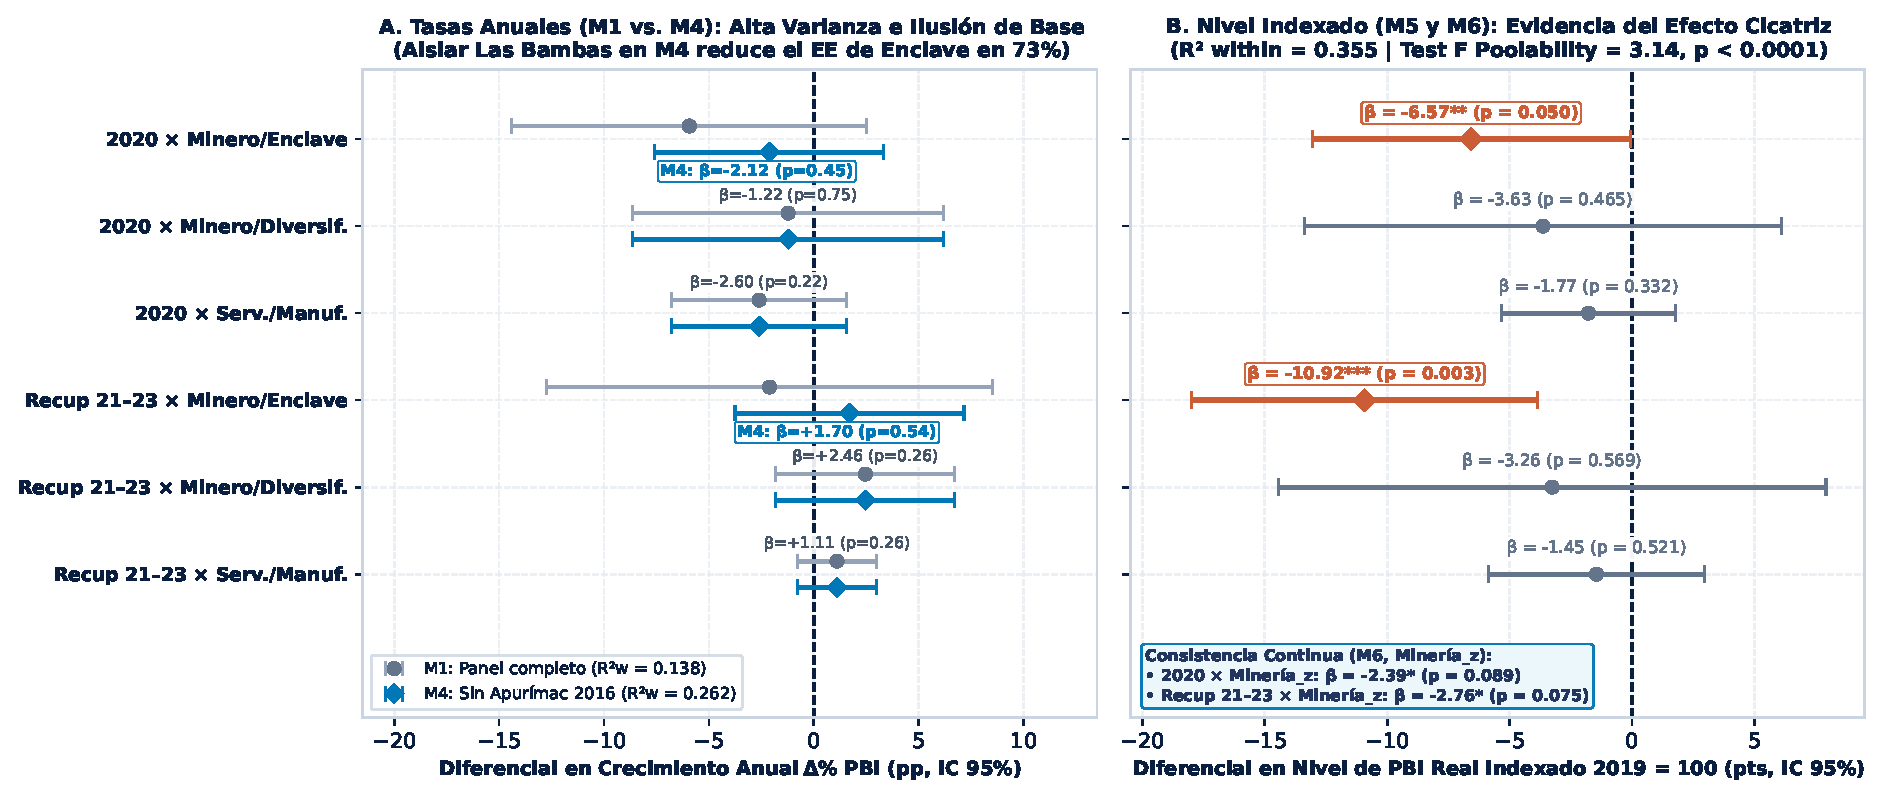
\includegraphics[width=0.90\textwidth,height=0.50\textheight,keepaspectratio]{figures/fig6_forest_plot_modelos.pdf}
\end{center}
\vspace{-0.24cm}
\begin{keybox}[left=2mm,right=2mm,top=0.8mm,bottom=0.8mm]
\scriptsize\RaggedRight
\textbf{Lección metodológica}: Evaluar choques estructurales mediante variaciones interanuales aisladas (Panel A) induce un \textbf{error Tipo II} (falso negativo). La especificación en nivel acumulado $\text{PIB}_{2019=100}$ (Panel B) revela la persistencia real del daño productivo.
\end{keybox}
\source{Intervalos de confianza al 95\% basados en errores estándar robustos agrupados por departamento.}
\end{frame}

